







\chapter{Introduction}


From the earliest days of quantum mechanics, the interaction of matter with electromagnetic radiation has been one of the central topics of physical research, and one of the main tools for the investigation of the world around us. Within this field, the ionization of atoms and molecules with light has been an incisive probe of atomic and molecular structure, and it has informed much of our understanding of the structure of matter. 

However, the naive picture of ionization, which roughly reads ``an atomic electron absorbs a photon and uses the energy to fly away,'' is misleadingly simple, and it hides much of the complex dynamics that ionization can encompass. For example, as the strength of the interaction increases, it enables multi-photon mechanisms that break out of the box of perturbative processes, with rich new dynamics that form a fresh new frontier between quantum and classical physics. This thesis works within this frontier.

We will work, in particular, with processes where an atom or molecule is subjected to a laser field with a long wavelength (so the photon energy is low, and many photons are required for each process) and the intensity is high (to supply the necessary photons). In this regime, the single-photon picture of ionization fades somewhat, giving way to a semiclassical picture of ionization where the electron is increasingly well described by trajectory language, though still retaining clear markings of quantum mechanics like interference between the outcomes from different trajectories and, in our case, complex-valued positions and times that stem from the application of trajectory language to situations that involve quantum mechanical tunnelling.

We will then examine this trajectory language, and explore the rich dynamics that it includes. How does quantum mechanical tunnelling emerge from a strong optical field? How can we describe it, starting from first principles, using trajectory language? How do complex time and complex positions arise in this context? What does it mean for a trajectory to have complex components, and how does such a trajectory interact with the~ion? These are some of the questions we will grapple with.

In addition, we will also examine some of the things that the photoelectron can do once ionized -- and, more specifically, the possibility for it to meet up with its parent ion and emit a sharp burst of high-frequency radiation. 



\section{A brief history of strong-field ionization}

The history of strong-field physics has been driven, to a large extent, by the development of lasers, which are uniquely able to provide the high intensities that drive physics out of the perturbative box. This pairing begins with T.\,H. Maiman's invention of the laser~\cite{ maiman_laser_1960}, which was used within five years of its creation to break ionization far from the single-photon, by ionizing xenon (with an ionization potential of $\SI{12.13}{eV}$) employing a ruby laser (with a photon energy of $\SI{1.79}{eV}$)~\cite{voronov_initial-multiphoton_1965, voronov_follow-up-multiphoton_1966}. Since that initial contact, laser developments have been a major driver of the field, and indeed later in this thesis we will help explain phenomena uncovered by new lasers, and prepare the way for the uses of future sources.


In terms of the ionization process, if it is possible for an electron to absorb six photons to leave the atom, then it is not such a stretch to ask for the absorption of an additional, seventh photon: can a photoelectron absorb from the field more energy than the bare minimum  it needs to fly away? As we shall see, the answer is a resounding yes -- a phenomenon known as above-threshold ionization (ATI)\,--, and at the end of this thesis we will see the photoelectron brokering the exchange of many thousands of laser photons. The start of this story, of course, is more modest, with the observation of electrons ionized from xenon with one more photon than strictly necessary~\cite{agostini_ati-initial_1979}. However, as technology improved, it became possible to observe the additional absorption of more and more photons~\cite{agostini_ati-development_1988} and, more surprisingly, to see the higher-order peaks become stronger than the low-order ones~\cite{agostini_ati-development_1988, petite_ati-nonperturbative_1987}.

This marks the beginning of non-perturbative strong-field physics, where the atom can no longer be considered to be driven by its own intrinsic dynamics with some minor influence by the radiation; instead, the laser field needs to be considered as an integral part of the dynamics, if not the major determinant in the electron's motion. This change in regime became evident with the observations of longer peak series~\cite{ schafer_ati-beyond-the-hhg-cutoff_1993}, nontrivial angular dependence for these peaks~\cite{baorui_ati-rings_1993}, strong dependences on the laser's polarization~\cite{corkum_long-wavelength-ati_1989}, and even long plateaus of photoelectron peaks~\cite{paulus_ati-plateau_1994}. Similarly, the generation of high-order optical harmonics with a broad, flat plateau~\cite{mcpherson_hhg-initial_1987, ferray_hhg_1988}, far from the exponential drop-down of perturbative theory, called for such a break from the usual theory.


The non-perturbative theory that explains these phenomena, on the other hand, had been ready and waiting for a long time. In fact, it also took but a few years from the invention of the laser for L.~V. Keldysh to lay the groundwork theory for the interaction with such pulses~\cite{keldysh_ionization_1965}, with work that introduced essential ideas that remain in use fifty years after its formulation~\cite{ dimauro_keldysh-plus-50_2014}. Keldysh's theory, later extended by F.~H.~M. Faisal and H. Reiss~\cite{faisal_multiple_1973, reiss_effect_1980}, as well as by  A.~M. Perelomov, V.~S. Popov and M.~V. Terent'ev~\cite{perelomov_ionization_1966, perelomov_ionization-II_1967, perelomov_ionization-III_1967}, introduced the idea of optical tunnelling: the idea that, if the frequency of light is low enough, it is best thought of as a slowly oscillating linear potential, $V(\vbr) = Fz\cos(\omega t)$, which combines with the atomic potential well to form a potential barrier that the electron then tunnels through.

This thesis works primarily within this tunnelling theory, the basics of which we will develop in section~\ref{sec:strong-field-basic-theory} below, and which has produced a long line of interesting advances over the years. For more details, we refer the reader to several good recent reviews~\cite{ popruzhenko_Keldysh_theory, long_Keldysh_theory, Popov_imaginary_time}.




\section{Applications}

The ionization of atoms and molecules in strong fields seems, at first glance, like a somewhat esoteric phenomenon, since the fields in question are often rather outside the range of any naturally occurring fields. However, this in itself provides a strong intrinsic motivation to study the behaviour of matter in this regime: the use of strong fields gives us a window into the behaviour of matter in situations where it is relatively untested, and, moreover, at the boundaries between well-understood behaviours, where rich and interesting dynamics have plenty of room.

In addition to its intrinsic interest, strong-field physics can tell us much about the structure and dynamics of the quantum mechanical systems that it probes, and it has produced several interesting windows on their behaviour. Some of these come from the direct observation of photoelectrons once they have come out, but many of them arise from recollision phenomena and hinge on effects that happen when the ionized photoelectron is brought back to its parent ion and interacts with it.

These phenomena include, for example, laser-induced electron diffraction~\cite{spanner_reading-diffraction-images_2004, yurchenko_laser-induced-rescattering_2004, blaga_imaging_2012} and holography~\cite{huismans_holography-2011}, where the recolliding electron diffracts on the nuclear and electronic structure of its parent ion, allowing us to image it both directly and via interference effects between the rescattered electron wave and the incident wavepacket. In this setting, the very high energy and momentum carried by the photoelectron during the recollision afford us a very fine-grained view of the molecule, in terms of both spatial and temporal resolution.

Similarly, many additional interesting ionization phenomena also depend on recollisions, including high-order above-threshold ionization, where electrons that rescatter off of the ion can achieve even higher energies than the usual tunnelling picture would predict~\cite{paulus_ati-plateau_1994}, and the surprisingly high efficiency of multiple ionization in strong laser fields~\cite{walker_nsdi_1994}, mostly through non-sequential multiple ionization mechanisms where one photoelectron returns to the ion and, in the ensuing recollision, ionizes one or more additional electrons.

Perhaps more importantly, the photoelectron's recollision with the ion is also a crucial way to generate radiation: as it passes by the nucleus, the photoelectron wavepacket interferes with the residual wavefunction that was left behind, making it oscillate and emitting a short, sharp burst of high-frequency radiation. This process is known as high-order harmonic generation (HHG), to which we will devote the second part of this thesis.

High-order harmonic generation is an important process, both scientifically and technologically, because it allows us to access time and length scales that have so far been unexplored. More specifically, it can be used to generate pulses of radiation that are so short~-- in the regime of a few femtoseconds, and even down to tens of attoseconds -- that we can now probe the motion of nuclei and electrons inside molecules with a time resolution that matches their dynamics~\cite{ calegari_phenylalanine_2014}. HHG provides a bright, coherent source of such pulses, without the need of a facility-scale experiment at a free-electron laser, and this is driving an entire new field known as attoscience~\cite{corkum_hhg-review_2007, krausz-ivanov_attosecond-review_2009}. In the second part of this thesis we will study and extend this process, providing ways to understand its relationship with spin angular momentum and to extend the available range of frequencies and time resolutions even further.


Much of strong-field physics, then, relies on models based on recollision phenomena, both in terms of the looser mental framework as well as in terms of the specific mathematics used in the analysis. In fact, a broad swathe of results can be analyzed quite well by simply using the ionization rates obtained via a simplified tunnelling model to seed electrons ionized at different times in the laser field, and subsequently propagating them on classical trajectories. 

However, the exact manner in which these trajectories arise from the Schrödinger equation is much less clear, and the success of the technique asks for a closer examination into their fundamental origin. The first part of this thesis deals largely with this problem: finding a trajectory language that describes the semiclassical post-ionization dynamics of the photoelectron, and obtaining these trajectories, in as complete a fashion as possible, directly from the Schrödinger fundamentals, rather than imposing them externally on the~formalism.




\section{Theoretical approaches to strong-field ionization}
\label{sec:strong-field-basic-theory}

Strong-field ionization is, in principle, well-understood, since it follows from the non-relativistic Schrödinger equation, with electrostatic Coulomb interactions between electrons and the nucleus, and with standard couplings to the driving radiation. (Occasionally one needs to include spin-orbit couplings~\cite{barth_spin-polarized_2013} or relativistic effects~\cite{milosevic_relativistic_2002}, but we will not need to do so here.) Thus, strong-field ionization largely falls within what Dirac aptly described in 1929~\cite{dirac_qm-many-electron_1929}:
%
\begin{quote}
The underlying physical laws necessary for the mathematical theory of a large part of physics and the whole of chemistry are thus completely known, and the difficulty is only that the exact application of these laws leads to equations much too complicated to be soluble.
\end{quote}
%
In essence, this means that all of the effects we will consider can in principle be deduced from the time-dependent Schrödinger equation (TDSE), and indeed if it were possible to integrate it directly, quickly and efficiently, for all relevant parameter ranges, then much of our work here would be unnecessary.

However, this is far from the case, and the numerical integration of the Schrödinger equation faces formidable challenges. Some of these are shared with the rest of atomic and molecular physics, and come from the unfavourable exponential scaling introduced by the presence of multiple electrons, for which even a moderate basis for the state space of each electron exponentiates to an unmanageable basis size for the full state space. Other challenges are more specific to strong-field physics, which involves electron motion over very large excursions (necessitating a large spatial grid) with very high momenta (calling for a small grid spacing), and with large energies (which require small timesteps).


These challenges are mostly surmountable, at least for specific situations and where the dynamics reduces to that of a single electron, and indeed there is a wide array of different methods to numerically solve the TDSE, which are well reviewed by A. Scrinzi in \citer{scrinzi_TDSE_chapter}, and which work for various different situations. These numerical solutions, however, tend to be computationally intensive, often to a prohibitive extent, and they are often overpowered for the insights we want to draw from them. In fact, we are often hindered in our understanding because even a full solution of the TDSE can be hard to analyze; as an example, it is often impossible to separate the contributions to ionization from different peaks of the field, even in situations where these contributions are clearly distinct and fulfil different roles in the dynamics. Thus, to retake Dirac's text,
%
\begin{quote}
It therefore becomes desirable that approximate practical methods of applying quantum mechanics should be developed, which can lead to an explanation of the main features of complex atomic systems without too much computation.
\end{quote}
%
In general, these approximate methods revolve around Keldysh's ideas about optical tunnelling, and in particular the Strong-Field Approximation, to which we now turn.



\subsection{Basic pictures of ionization}
In general, there are two basic mental pictures of strong-field ionization, the multiphoton picture and the tunnelling picture, which are best explained graphically, as shown below.


\begin{figure}[h]
  \centering
  \subfigure[Multiphoton picture]{
    \label{f1-multiphoton-picture}
    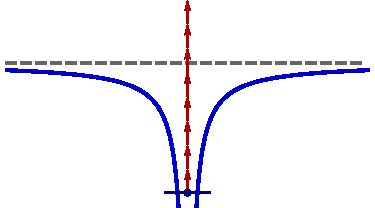
\includegraphics[scale=1]{1-Introduction/Figures/figure1Aa.pdf}
  }
  \hspace{3mm}
  \subfigure[Tunnelling picture]{
    \label{f1-tunnelling-picture}
    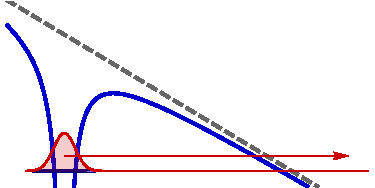
\includegraphics[scale=1]{1-Introduction/Figures/figure1Ab.pdf}
  }
  \caption[Basic pictures of strong field ionization]{
  Basic pictures of strong field ionization: \protect\subref{f1-multiphoton-picture} the multiphoton picture, in which an electron absorbs multiple energy quanta from the external field, and \protect\subref{f1-tunnelling-picture} the tunnelling picture, in which the external potential $V_L = -Fx\cos(\omega t)$ tilts the potential landscape enough to form a barrier the bound wavefunction can tunnel through.
  }
\label{f1-basic-pictures}
\end{figure}

As shown by Keldysh, these two pictures are actually two different sides of the same coin, and they are only truly valid  as limiting behaviours. More concretely, if we consider the ionization of a system with ionization potential $I_p=\frac12 \kappa^2$ by a monochromatic field of the form $F\cos(\omega t)$, with angular frequency $\omega$ and electric field amplitude $F$, then much of the behaviour is governed by the Keldysh adiabaticity parameter,
\begin{equation}
\gamma = \frac{\kappa \omega}{F} = \sqrt{\frac{I_p}{2U_p}},
\label{e1-keldysh-parameter}
\end{equation}
often called simply the Keldysh parameter. Here we assume that the field is `slow', or that the target is `hard', in the sense that $\omega\ll I_p$, and it takes multiple photons to ionize the system. 

However, there is a separate timescale to consider -- the time it takes for the electron to tunnel through the barrier at the peak of the field, which can be estimated using quasi-static arguments~\cite{landau_QM} as $\tau_\mathrm{tunn}\sim\kappa/F$. Thus, if the field changes slowly enough to permit appreciable tunnelling, in the regime of low $\gamma\propto\omega$, the behaviour is mostly in the tunnelling picture. Conversely, if the field is too fast or too weak for this, and $\gamma$ stays high, then the ionization mostly displays multi-photon picture features that can mostly be explained through a perturbation-theory viewpoint.

Alternatively, the Keldysh parameter can also be seen as the relationship between the energy scales of the ground state energy, $-I_p$, and the ponderomotive potential \mbox{$U_p=F^2/4\omega^2$}, which is the average oscillatory energy of an electron moving in the field. Thus, at low $\gamma$, the oscillatory motion has much more energy than that required to ionize the electron in the first place, and vice versa.




\subsection{A quick note on units}
Throughout this thesis we will use the atomic system of units, unless otherwise noted. This system of units is fixed by taking the essential dynamical quantities of atomic physics as unity,
\begin{equation}
\hbar = m_e = e^2 = \frac{1}{4\pi\eps_0} = 1,
\end{equation}
and it is reviewed more fully in Appendix~\ref{chap:atomic-units}. Also note that, to avoid confusion between energies and electric fields, we denote the latter with the letter $F$ throughout.%
\footnote{%
Since we're discussing style, this is a good place to apologize for the use of the plural first person throughout this thesis. This is relatively awkward, but the singular first person is even worse, and passive constructions are the bane of readability. The author invites the reader to include his or herself in this scientific `we', or (if that is uncomfortable) to include the immortal F.D.C. Willard in that plural first~person.
}



\subsection{Essential approximations}

To make our treatment more concrete, we now need to start approximating, since the full Schrödinger equation requires the brunt of a numeric integrator to handle in full. There are several key approximations that we need to make, with varying degrees of generality (and some of which we will discard later on).

\begin{itemize}
\item We will work throughout using non-relativistic quantum mechanics, an approximation that states that the laser field may well move the electrons fairly violently, but it will keep them at a reasonable fraction of the speed of light; this sets an upper limit of field strength at about $\SI{e16}{W/cm^2}$ (at which field strength most species get multiply ionized), and we will stay below that regime. 

In chapter~\ref{chap:nondipole-HHG} we will come somewhat close to relativistic velocities but, for the observables of interest there, a full relativistic treatment is not necessary.

\item In addition, we will also work, with the exception of chapter~\ref{chap:nondipole-HHG}, within the dipole approximation. In general, if we have a non-relativistic electron subject to an atomic potential $V(\vbr)$ and interacting with a laser field of vector potential $\vba(\vbr,t)$ of the external field (which we always take in the radiation gauge, and which relates to the electric field via $\vbf(\vbr,t)=-\frac{\partial \vba}{\partial t}(\vbr,t)$), then the minimal coupling hamiltonian reads
\begin{equation}
\hat H = \frac{1}{2} \left(\vbp +\vba(\vbr,t)\right)^2 + V(\vbr).
\end{equation}
In general, the spatial variation of the vector potential $\vba(\vbr,t)$ will be on the order of the wavelength $\lambda$ of the laser; the shortest such wavelength that we will consider will be $\SI{400}{nm}$, on the order of $\SI{1000}{\au}$ In a strong field context, the electron can make some very long excursions, but these will typically be smaller than the wavelength (and, moreover, will tend to be orthogonal to the propagation direction). 

%%%Note hackish \au-period above

This means, then, that we can safely replace the vector potential with its value at the nucleus of our atom of interest (or, with molecules, at the nuclear centre of charge), getting a hamiltonian of the form 
\begin{equation}
\hat H = \frac{1}{2} \left(\vbp +\vba(\vb 0,t)\right)^2 + V(\vbr).
\label{e1-velocity-gauge-hamiltonian}
\end{equation}
We will term hamiltonians of this form as being in the \textit{velocity gauge}, since the interaction hamiltonian in $\hat H = \frac{1}{2} \vbp^2 + V(\vbr) + \vba(\vb0,t)\cdot\vbp +\vba(\vb0,t)^2$ couples directly to the velocity operator $\vbp$.

Working in the dipole approximation allows us to change to a more convenient gauge, which we will term the \textit{length gauge}, via the unitary transformation $\hat U=e^{-i\vba(\vb0,t)\cdot\hat\vbr} e^{-\frac i2\int \vba(\vb0,t)^2\d t}$, which gives the length-gauge hamiltonian as 
\begin{equation}
\hat H = \frac{1}{2} \vbp^2 + V(\vbr) - \vbr\cdot\vbf(\vb0,t).
\label{e1-length-gauge-hamiltonian}
\end{equation}

As a separate effect, within the dipole approximation the vector potential has no spatial dependence, which means that its magnetic field $\vb B(\vbr,t)=\nabla \times \vba(\vbr,t)$ necessarily vanishes. In chapter~\ref{chap:nondipole-HHG} this will push us to discard the dipole approximation but unless one works at extremely high intensities or at very long wavelengths (which, as we shall see, can also cause a breakdown of the dipole approximation), the magnetic field is negligible.  (Finally, for notational convenience, and unless it is required for clarity, we will henceforth drop the spatial indicator $\vb0$.)





\item While this is seldom made explicit in more recent strong-field physics, most of what follows requires that the laser pulse be short enough for the laser pulse to end before the photoelectron can leave the focus, which in practice needs pulses shorter than some hundreds of femtoseconds. If this fails, then one needs to consider the effect on the photoelectron's momentum of the edge of the focus, which will drastically change the structures of interest; moreover, a long pulse can quite easily saturate the ionization. Pulses of this length are, of course, perfectly accessible to modern light sources and indeed they are required to attain the intensities at play.


\item Moreover, we will work in the clamped-nucleus approximation, both for the handling of atoms and with molecules, leaving the nuclei at their equilibrium separation. 
\end{itemize}


In addition to these approximations, most of strong-field physics works rather well under what is known as the Single-Active Electron (SAE) approximation, which is implicit in both the hamiltonians in \eqref{e1-velocity-gauge-hamiltonian} and \eqref{e1-length-gauge-hamiltonian} above: in general, much of strong-field phenomena can be understood rather well by assuming that each electron acts independently, neglecting the effects of electron correlation and exchange, and that the rest of the electrons in the system act only to provide the effective potential $V(\vbr)$.

The single-active electron approximation is remarkably effective, mostly due to the fact that a strong laser field will typically take the active electron far away from the rest of the system rather quickly, and it will afterwards be dynamically very different from the remaining electrons, even if it comes back to do diffractive imaging. In fact, it works well even in non-sequential double ionization via recollision mechanisms, where the pre-recollision dynamics can essentially be done with a single active electron.

On the other hand, there are multiple reasons to go beyond the single-active electron paradigm, which we will recount in more depth in chapter~\ref{chap:multi-channel}, especially driven by the fact that the ion can be left in an excited state after the pulse is over. While this can happen through single-electron mechanisms, essentially by removing an electron from an orbital below the highest-occupied one, there is increasing evidence that electron correlation can play a role in this process. 

To accommodate for this we will build a multi-electron theory in chapter~\ref{chap:R-matrix} and examine it in more detail in chapters~\ref{chap:multi-channel} and~\ref{chap:complex-space-potentials}, before reverting to single-electron phenomena for the rest of the thesis. For the moment, we will show a sketch of the Strong-Field Approximation, as developed by Keldysh, within the single-active electron approximation.



\subsection{The Strong-Field Approximation}


This leaves us, then, with the final core approximation of analytical strong-field physics, the stipulation that after the ionization step the photoelectron is at the mercy of the radiation field, if it is strong enough, and that the electric field of the ion plays, at most, a perturbative role. This can be done in a number of different ways, giving slightly different approaches, many of which are grouped under the name of the Strong-Field Approximation, despite their (sometimes substantial) differences. We will not delve into the various formulations of this approximation, which has been reviewed elsewhere~\cite{popruzhenko_Keldysh_theory, galstyan_sfa-reformulation_2016}; instead, we will give a sketch of Keldysh's original approach and then discuss the generalities of the overall method.


We begin, then, with the Schrödinger equation in the presence of the laser field, in the~form
\begin{equation}
i\frac{\d}{\d t}\ket{\psi(t)}
=\hat H \ket{\psi(t)}
=\left[ \frac12 \vbp^2 + V(\vbr) + \vbr\cdot \vbf(t) \right]\ket{\psi(t)},
\label{e1-sfa-tdse}
\end{equation}
where we are assuming a single active electron and working in the length gauge. As an initial condition, we take the electron to sit in the ground state of the system, $e^{-iE_gt}\ket{\psi_g}$, before the pulse starts. The core of the Strong-Field Approximation, as a method, is to assume, first, that this is the only bound state of the system that will contribute to the dynamics (though, again, that can be relaxed~\cite{perez-hernandez_sfa-plus_2009}). We postulate, then, an Ansatz of the form
\begin{equation}
\ket{\psi(t)} = e^{-iE_g t}\ket{\psi_g} + \ket{\psi_\mathrm{out}(t)},
\label{e1-keldysh-ansatz}
\end{equation}
where $\ket{\psi_\mathrm{out}(t)}$ is the outgoing continuum electron.

(Here it is important to remark that, although physics should in principle be fully gauge-indepen\-dent, as will be much of our handling of $\ket{\psi_\mathrm{out}(t)}$, the Ansatz in \eqref{e1-keldysh-ansatz} is not gauge independent, since we are performing an approximation by trimming down the complete set of bound states to just a single component, so this is actually a different approximation if performed in the velocity gauge~\cite{galstyan_sfa-reformulation_2016}, which can correspondingly lead to different results.)

In addition to the bound-state Ansatz in \eqref{e1-keldysh-ansatz}, the Strong-Field Approximation also completely ignores the role of the atomic potential $V(\vbr)$ once the electron is in the continuum, so the outgoing wave-packet obeys the laser-only Schrödinger equation,
\begin{equation}
i\frac{\d}{\d t}\ket{\psi_\mathrm{out}(t)}
=\left[ \frac12 \vbp^2 + \vbr\cdot \vbf(t) \right]\ket{\psi_\mathrm{out}(t)}.
\end{equation}
This equation can, fortunately, be solved exactly,%
%
\footnote{
Incidentally showing that exact solutions in quantum mechanics are not confined to the harmonic oscillator as the go-to system. Instead, it is also perfectly possible to solve for a particle in a uniform force field, even with an arbitrary time dependence.
}
%
and moreover it admits solutions which are plane waves throughout, known as Volkov states. These are given by
\begin{equation}
\braket{\vbr}{\Psi^\mathrm{(V)}_{\vbp}(t)}
=
\frac{1}{(2\pi)^{3/2}}
e^{i(\vbp+\vba(t))\cdot\vbr}
e^{-\frac i2 \int_{T}^t \left(\vbp+\vba(\tau)\right)^2 \d\tau}
,
\label{e1-volkov-wavefunctions}
\end{equation}
and they have a kinetic momentum $\vbv(t)=\vbp+\vba(t)$ which oscillates with the laser field, accruing phase via the kinetic energy $\frac12 \vbv(t)^2$. 

The Volkov states are excellent building blocks, and we will later modify them to account for the Coulomb field of the ion, to give the eikonal-Volkov states of chapter~\ref{chap:R-matrix}, and to include the magnetic field of the driver, giving us non-relativistic non-dipole Volkov states in chapter~\ref{chap:nondipole-HHG}. For the moment, though, we keep them as they are.


This means that we can re-phrase our Ansatz in the form
\begin{equation}
\ket{\psi(t)} 
= 
e^{-iE_g t}\ket{\psi_g} 
+ \int \d\vbp \,a(\vbp,t) \volkov{\vbp}{t}, 
\label{e1-keldysh-full-ansatz}
\end{equation}
where $a(\vbp,t)$ is the time-dependent amplitude of each Volkov state, which we need to solve for. This Ansatz comes with the assumption that $\braket{\psi_g}{\Psi^\mathrm{(V)}_{\vbp}(t)} \approx 0$ for all canonical momenta $\vbp$, which is clearly wrong, but it does a good job at specifying the separation of the active Hilbert space into a bound-state component and a field-driven continuum. 

We have, then, a full Ansatz for the wavefunction, \eqref{e1-keldysh-full-ansatz}, which now allows us to put it into the Schrödinger equation to get the dynamics. Since we have included most of the dynamics already into our bound and continuum components, the Schrödinger equation simplifies a good deal, to give
\begin{align}
\left(
i\frac{\d}{\d t}
-\hat H
\right)\ket{\psi(t)}
& =
-\vbr\cdot\vbf(t) e^{-iE_g t}\ket{\psi_g}
+ \int \d\vbp \,
\left( 
i\frac{\partial a}{\partial t}(\vbp,t) 
-V(\vbr)a(\vbp,t)
\right)
\volkov{\vbp}{t}
,
\end{align} 
or, projecting on the Volkov state $\volkov{\vbp}{t}$,
\begin{align}
i\frac{\partial a}{\partial t}(\vbp,t)
& =
e^{-iE_g t}\matrixel{\Psi_{\vbp}^\mathrm{(V)}(t)}{\vbr\cdot\vbf(t)}{\psi_g}
%\nonumber \\ & \qquad
+\int \d\vbp' \,
a(\vbp',t)
\matrixel{\Psi_{\vbp}^\mathrm{(V)}(t)}{V(\vbr)}{\Psi_{\vbp'}^\mathrm{(V)}(t)}
.
\end{align}
Here we perform our final approximation by neglecting the second term, which represents continuum-continuum transitions induced by the atomic potential, i.e. scattering on the atomic core, which is again outside of the SFA (though it can be put back in to account for rescattered electrons in ATI~\cite{milosevic_ISFA-standard_2007}).

The Schrödinger equation thus reduces to a simple ordinary differential equation, and its solution can be stated simply in terms of a time integral in the form
\begin{align}
a(\vbp)
& =
-i
\int_{-\infty}^{\infty} \!
e^{iI_p t+\frac i2 \int_{\tn}^{t} \left(\vbp+\vba(\tau)\right)^2 \d\tau}\matrixel{\vbp+\vba(t)}{\vbr\cdot\vbf(t)}{\psi_g}
\, \mathrm dt
.
\label{e1-keldysh-integral-result}
\end{align}
(Here we have set $I_p=-E_g>0$ for convenience, extracted the explicit phase and plane wave $\ket{\vbp+\vba(t)}$ from the Volkov state, and asked for the amplitude at $t\to\infty$ after the pulse is over.)  This is, essentially, the main final answer from the Keldysh-style SFA, though we will analyse it further below. 




\subsection{Imaginary time and trajectory language}
The result in \eqref{e1-keldysh-integral-result} closes an impressive gap, by taking the full TDSE and reducing it to a single integral per final momentum $\vbp$, so it can be queried directly and easily. However, it can still be simplified considerably by suitably modifying the integration path into the complex plane. 

We will analyse  this in more detail in chapter~\ref{chap:R-matrix}, but it is easy to see that the integral is highly oscillatory, since it includes a factor of $e^{iI_pt}$ being integrated on the scale of several laser cycles, and we are working in the regime where $\omega \ll I_p$. (There is an additional average factor of $e^{iU_pt}$ coming from the kinetic term of the phase, which is even larger for $\gamma<0$, but this only increases the severity of the problem.) This makes the numerical integration of \eqref{e1-keldysh-integral-result} challenging, since one the final value comes through heavy cancellations, so one needs to compute each lobe to very high accuracy to get only moderate precision on the final result, or use sophisticated integration algorithms that attempt to account for this.

The most efficient approach, however, is to recur to the tools of complex analysis in the form of the \textit{saddle-point approximation}. We will explain this in depth in chapter~\ref{chap:R-matrix} (and there are good reviews in Refs.~\citealp{popruzhenko_Keldysh_theory} and \citealp{Popov_imaginary_time}), but the essence is that one can modify the integration path of \eqref{e1-keldysh-integral-result} away from the real axis in a way that turns the oscillatory exponential 
\begin{equation}
e^{-iS(\vbp,t)} = \exp({iI_p t+\frac i2 \int_{T}^{t} \left(\vbp+\vba(\tau)\right)^2 \d\tau})
\label{e1-sfa-action}
\end{equation}
into a series of gaussian bumps with a flat phase, which essentially reduce to the contributions from a discrete series of points at the top of those gaussians. These are the saddle points $\ts$ of the exponent $S(\vbp,t)$, which satisfy the core saddle-point equation
\begin{equation}
\frac{\partial S}{\partial t}(\vbp,\ts) = 0,
\label{e1-initial-saddle-point-equation}
\end{equation}
which make the phase stationary. In addition, a quick look at $S(\vbp,t)$ shows that it is the kinetic action of an electron in the laser field, so the condition \eqref{e1-initial-saddle-point-equation} is a form of the principle of stationary action (and, indeed, the connection to Feynman's path integral formalism can be made explicit and rigorous~\cite{salieres_quantum_orbits}).

The result, then, is an approximation to the ionization yield $a(\vbp)$ in the form of the sum of the integrand over a discrete collection of saddle points $\ts$, chosen by the ability to deform the integration path to reach them, in the form
\begin{equation}
a(\vbp)
=
\sum_{\ts}
\sqrt{\frac{2\pi}{i\partial^2 S/\partial t^2(\vbp,\ts)}}
e^{-iS(\vbp,\ts)} 
\matrixel{\vbp+\vba(\ts)}{\vbr\cdot\vbf(\ts)}{\psi_g}
.
\label{e1-saddle-point-result}
\end{equation}
More appealingly, this form also gives us a compelling physical picture which we can just read off: the electron, originally in the ground state $\ket{\psi_g}$, performs a transition at a time $\ts$ through the laser coupling $\vbr\cdot\vbf(\ts)$ to a continuum state with initial kinetic momentum $\vbp+\vba(\ts)$ (which, moreover, can be shown to have vanishing velocity along the laser polarization), and it then propagates classically accruing action exactly as a free electron in the laser field, via
\begin{equation}
S(\vbp,t) =-I_p t-\frac 12 \int_{\tn}^{t} \left(\vbp+\vba(\tau)\right)^2 \d\tau
,
\label{e1-sfa-action-real}
\end{equation}
with a factor of $\sqrt{\frac{2\pi}{i\partial^2 S/\partial t^2(\vbp,\ts)}}$ as a remainder of the time integration. There will be, in principle several  of these trajectories, and we simply add their probability amplitudes as~usual. Each such factor, in turn, can be directly interpreted as coming from a single trajectory ionized at time $\ts$ and evolving with velocity $\vbv(t)=\vbp+\vba(t)$.


There is a problem, of course, and it is that the saddle-point times $\ts$ generally do not lie on the real axis, and that therefore we do need to modify the integration path in \eqref{e1-keldysh-integral-result} to reach them. This is not very problematic when we are talking about the amplitudes -- they are just some mathematical function in a convenient and compact form~-- but it raises some serious conceptual issues when we attempt to understand each individual term in the sum as corresponding to a classical trajectory. What does it mean for an electron to be ionized at a complex time? What is the physical meaning of that ionization time, and can it be measured experimentally? What does the trajectory look like, and what does it mean physically? These questions have plagued the field since Keldysh first raised the issue~\cite{keldysh_ionization_1965}, and they do not yet have satisfactory answers.


The usual way of understanding the complex ionization times $\ts$ is to get away from them as fast as possible: that is, if we need to visualize the passage of time for the electron from its ionization at $\ts = \tn +i\tauT$, we normally first take it straight down to the real part $\tn=\Re(\ts)$, and we can then take it along the real axis more normally, as shown~in~\reffig{f1-initial-contour}.

\begin{figure}[ht]
  \centering
  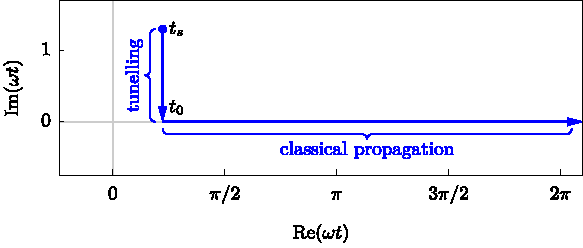
\includegraphics[scale=1]{1-Introduction/Figures/figure1B.pdf}
  \caption[Standard contour from the complex ionization time $\ts$ to its real part $\tn$ and then along the real axis]{
  Standard contour for understanding trajectories in complex time going from the complex ionization time $\ts$ to its real part $\tn$ and then along the real axis until the final detection at a large, real time.
  }
\label{f1-initial-contour}
\end{figure}

This has the advantage of clearly delineating the roles of each part of the contour, and it matches rather well our understanding of how tunnel ionization should work: the downwards part of the path takes place in complex time, so $S(\vbp,t)$ will be complex and $e^{-iS(\vbp,t)}$ will be a strong modulation on the amplitude; similarly, on the classical propagation part the velocity and action are now real, and everything behaves much as Feynman originally described it, with a (restricted) set of classical trajectories that are eventually added with probability amplitude $e^{-iS(\vbp,t)}$. Even better, the `tunnel exit' in this formalism, $\int_{\ts}^{\tn}\left[\vbp+\vba(t)\right]\d t$, can be shown to reduce to the usual $I_p/F$ in the quasistatic $\gamma \ll 1$~limit.


In addition to being very appealing, this classical understanding very often works, and can be very effective. One very pervasive way to implement this is to use the above formalism purely to obtain the tunnelling rate down to the real axis, and then to completely forget about quantum mechanics: to consider \eqref{e1-saddle-point-result} as describing the emergence at time $\tn$ of an electron with zero longitudinal velocity with probability
\begin{equation}
\left|
\sqrt{\frac{2\pi}{i\partial^2 S/\partial t^2(\vbp,\ts)}}
\matrixel{\vbp+\vba(\ts)}{\vbr\cdot\vbf(\ts)}{\psi_g}
\right|^2
\times
e^{2\Im\left(S(\vbp,\ts)\right)} 
,
\end{equation}
and then to propagate these trajectories classically, either under the laser driving only or also including the effect of the ionic potential.%
\footnote{%
Generally, this is changed to the ADK rates~\cite{ammosov-delone-krainov-1986}, to include the effect of the Coulomb potential during the tunnelling step, but this does not change the fundamentals.
}
This method, known generally as the classical-trajectory Monte Carlo (CTMC) approach, can be very effective, and we will meet it again in chapter~\ref{chap:LES-NZES}.

However, this method, and others like it, is essentially only a model: it is grounded in a calculation from the TDSE, but eventually it departs from it and works by analogy, introducing the constructs that look appropriate (like, for example, the effect of the ionic potential on the trajectory) in a form that fits into its environment, and hoping for the result to match experimental measurements. As a model, the CTMC approach has a number of successes (as do its several analogues), but it is very thinly grounded on the Schrödinger equation. 

This is, in a way, one of the key problems that this thesis tackles: can one derive a trajectory-based model, which allows one among other things to describe the interactions with the ion's potential, directly from the Schrödinger equation, and without proceeding by analogy or similar leaps? As we will see, this is indeed possible, but it comes at the cost of having a complex-valued trajectory once the time reaches the real axis. Moreover, this imaginary component of the position is retained all the way to the detector, it has a very strong effect on the interaction with the ion, and it ultimately makes the standard contour shown in \reffig{f1-initial-contour} inadmissible and essentially meaningless. 

In essence this is because the imaginary component of the position combines with the Coulomb potential of the ion, $-1/\sqrt{\vbr^2}$, to produce branch cuts in the complex time plane that severely restrict the paths the trajectory can take, and we will show how to navigate these branch cuts to obtain suitable paths in the complex time plane. This method will then allow us to explain intricate structures that appear in the low energy region of ATI spectra. More recently, the inclusion of this imaginary component of the position has also been shown to be crucial in explaining higher-energy phenomena~\cite{keil_branch-cuts_2016}, in the intersection of direct and rescattered ATI electrons, with our method of branch cut navigation successfully allowing the evaluation of correct trajectories, at the expense of the foot $\tn$ of the standard contour as a central concept of the theory.








\subsection{Including the Coulomb field of the ion}
Coming back to the Keldysh result \eqref{e1-saddle-point-result}, it is also important to remark that, for all its conceptual and quantitative successes, the Keldysh theory does have some serious limitations. One of them is the limitation to relatively weak fields limited by $F\ll \SI{1}{\au}$, so the theory only works in the tunnelling regime, where the barrier still exists, and it fails for over-the-barrier ionization where the potential in \reffig{f1-tunnelling-picture} dips below the energy of the ground state, liberating the wavefunction and ensuring very swift and complete ionization. 

(In general, however, this is not too hindering a limitation, since if a pulse goes above that intensity then the leading edge, which still falls within the tunnelling limits, is very likely to saturate the ionization, presenting the higher fields in the middle of the pulse with a harder target with a higher ionization potential that is often still inside the tunnelling regime, now modified to $F\ll (2I_p)^{3/2}$.)


More seriously, on the other hand, the Keldysh theory is limited to only short-range potentials, and it produces very poor quantitative results when applied to charged systems with an asymptotic Coulomb potential, often out by several orders of magnitude (even if the shape of the spectrum is relatively accurate). As such, one of the key goals of the theory of strong-field physics is to have an analytical theory -- ideally sharing as much of the SFA's conceptual and computational simplicity -- that includes this Coulomb potential.


Several approaches have extended the Keldysh method to include the Coulomb potential, most notably by A.~M. Perelomov, V.~S. Popov and M.~V. Terent'ev~\cite{perelomov_ionization_1966, perelomov_ionization-II_1967, perelomov_ionization-III_1967} for a nonzero charge, known as the PPT model, and later simplified by M. Ammosov, N. Delone and V. Krainov~\cite{ammosov-delone-krainov-1986}, dealing with arbitrary initial states, giving the so-called ADK rates that extend well to the case of molecules~\cite{tong_mo-adk_2002}. However, extending these methods to observables beyond the ionization rate has proved challenging, and though there are several interesting methods available there is as yet no completely satisfactory theory for~this.




\subsubsection{PPT methods}
The core method for including the Coulomb field into the SFA ionization rates was provided by Perelomov et al. in \citer{perelomov_ionization-II_1967}, and it can be simplified a good deal by phrasing it in trajectory language~\citer{perelomov_ionization-III_1967}, which can then be modified to include the Coulomb field in a relatively ad-hoc way. Using integration by parts, one can rephrase the action \eqref{e1-sfa-action} as
\begin{align}
S(\vbp,t) 
&=
-I_p t+\frac 12 \int_{T}^{t} \left[\vbv(\tau)^2 + \vbr(\tau)\cdot \dot{\vbv}(\tau) \right] \d\tau
\nonumber \\ &=
-I_p t + \int_{T}^{t} \left[\frac 12 \vbv(\tau)^2 - \vbr(\tau)\cdot \vbf(\tau) \right] \d\tau
,
\label{e1-sfa-action-lagrangian}
\end{align}
where $\vbr(t)=\int_{t_\mathrm{ref}}^{t}\left[ \vbp+\vba(\tau)\right] \d\tau$ and $\dot\vbv(t) = \frac{\d\vba}{\d t} =-\vbf(t)$, and this is explicitly in the form of a lagrangian function $L=\frac 12 \vbv(\tau)^2 - \vbr(\tau)\cdot \vbf(\tau)$ with an explicit potential. To include the Coulomb potential here, and working in analogy to our original hamiltonian from \eqref{e1-sfa-tdse}, we can simply expand this to
\begin{equation}
L=\frac 12 \vbv(\tau)^2 - \bigg[ \vbr(\tau)\cdot \vbf(\tau) +V(\vbr(\tau)) \bigg].
\end{equation}
This requires some amount of care, since integrating $\int V(\vbr(\tau))\d\tau$ can produce infinities coming from the $1/r$ singularity at the origin, but in general these can be appropriately regularized. However, it is relatively challenging to extend this to a full photoelectron momentum spectrum, and the theory misses some non-adiabatic tunnelling effects, which come from the temporal variation of the barrier, for Coulomb potentials. As such, in general the use of PPT methods in the recent literature is mostly seen in calculations of total rates or, through the extension to ADK~\cite{ammosov-delone-krainov-1986} and molecular ADK~\cite{tong_mo-adk_2002} to arbitrary atomic and molecular states, respectively, for the calculation of instantaneous tunnelling rates, down to the tunnelling `foot' of the integration, for CTMC calculations. 



\subsubsection{Coulomb-Corrected Strong-Field Approximation}
The ideas of the PPT method reach their full fruition in what's generally known as Coulomb-corrected SFA methods (CCSFA), first introduced by S.~V. Popruzhenko and co-workers in Refs.~\citealp{CCSFA_initial_short, CCSFA_initial_full, popruzhenko_ccsfa-arbitrary-frequency_2008, popruzhenko_multiphoton_2009}. In essence, these methods take the SFA expression for the ionization amplitude, 
\begin{equation}
a(\vbp)
=
\sum_{\ts}
\sqrt{\frac{2\pi}{i\partial^2 S/\partial t^2(\vbp,\ts)}}
e^{-iS(\vbp,\ts)} 
\matrixel{\vbp+\vba(\ts)}{\vbr\cdot\vbf(\ts)}{\psi_g}
,
\backtag{e1-saddle-point-result}
\end{equation}
and retain its form, modifying only the action, both in terms of its explicit form as well as the trajectory that it is evaluated on. 

In general, this usually means expanding to first order about the laser-driven system, with trajectory $\vbr_0(t)=\int_{t_\mathrm{ref}}^{t}\left[ \vbp+\vba(\tau)\right] \d\tau$  and the action \eqref{e1-sfa-action-lagrangian}, to include the Coulomb potential in the latter via
\begin{align}
S_{\textsc{ccsfa}}(\vbp,t) 
&=
-I_p t + \int_{T}^{t} \left[\frac 12 \dot{\vbr}(\tau)^2 - \vbr(\tau)\cdot \vbf(\tau) \right] \d\tau
-\int_{T}^t V(\vbr(\tau))\d\tau
,
\label{e1-ccsfa-action-lagrangian-coulomb}
\end{align}
and to expand the trajectory to $\vbr(t) = \vbr_0(t) + \vbr_1(t)$, where $\vbr_0(t)$ is the laser-driven trajectory and, in lieu of the full equation of motion
\begin{equation}
\ddot \vbr(t) = -\vbf(t) -\frac{Z\vbr(t)}{\|\vbr(t)\|^3},
\label{e1-ccsfa-equation-of-motion-full}
\end{equation}
it is often sufficient to take only a first-order correction,
\begin{equation}
\ddot \vbr_1(t) = -\frac{Z\vbr_0(t)}{\|\vbr_0(t)\|^3}.  \phantom{-\vbf(t)}
\label{e1-ccsfa-equation-of-motion-first-order}
\end{equation}
These methods can be put together in different combinations (so, for example, the correction to the action can be left only as $-\int_{T}^t V(\vbr_0(\tau))\d\tau$, or the corrections to the trajectory may be discarded), depending on the conditions of the problem.

In addition to this, the CCSFA methods typically require the canonical momentum $\vbp'$~at ionization to be different to the final momentum $\vbp$ at the end of the pulse, because the equations of motion (\ref{e1-ccsfa-equation-of-motion-full}, \ref{e1-ccsfa-equation-of-motion-first-order}) do not conserve the canonical momentum as the laser-only evolution does. This poses a problem, because when we evaluate a photoelectron momentum spectrum we usually fix a final momentum $\vbp$, and we want to calculate its ionization amplitude; this is an inverse problem (given a final momentum, find the initial conditions that lead to it), but the CCSFA postulates are posed as a forward one (given initial conditions they produce the final momentum). This can be solved via a `shotgun' approach to the momentum, by seeding a large number of initial conditions and seeing what their final momentum is. The procedure requires some care (such as when calculating the interference between trajectories whose final momenta almost, but do not quite, match), but it can be done with a framework that is essentially as efficient and flexible as the original SFA.


A somewhat more problematic issue, however, is the setting of the initial conditions for the trajectories. The SFA trajectory language tells us a fair amount about the trajectories, most notably through their velocity $\vbv(t)=\vbp+\vba(t)$, but it is mute about where the trajectory starts. This is required information to compute the trajectory via the equations of motion~(\ref{e1-ccsfa-equation-of-motion-full}, \ref{e1-ccsfa-equation-of-motion-first-order}), and it is similarly necessary to compute the Coulomb action in~\eqref{e1-ccsfa-action-lagrangian-coulomb} even if only the zeroth-order trajectory is used, via $-\int_{T}^t V(\vbr_0(\tau))\d\tau$. 

Thus, the CCSFA method requires an initial condition to be put in externally, which can be done but it means that the formalism is firmly on the class of a model that proceeds by analogy. It is certainly very successful, and it correctly explains, among other things, the Coulomb-enhanced ionization rate~\cite{popruzhenko_ccsfa-arbitrary-frequency_2008} and the breaking of the SFA's excessive symmetry in an elliptically polarized field~\cite{CCSFA_initial_short, CCSFA_initial_full}. However, it does not derive directly from a TDSE, which makes it desirable to find an analogous theory that does proceed from first principles and arrives at a similar trajectory-based intuitive understanding of the ionization process.






\subsubsection{Coulomb-Volkov Approximation}
On a separate approach to the inclusion of the Coulomb potential is what is known as the Coulomb-Volkov Approximation (CVA)~\cite{jain_coulomb-volkov_1978,cavaliere_coulomb-volkov_1980}, which essentially consists of replacing the Volkov states in the SFA results -- both the integral version~\eqref{e1-keldysh-integral-result}, and from there to the saddle-point result~\eqref{e1-saddle-point-result} -- with Coulomb-modified scattering waves that incorporate spatial aspects of the Coulomb waves $\ket{\Psi_{\vbp}^{(-)}}$ in addition to Volkov-state behaviour; more specifically, of the form
\begin{align}
\braket{\vbr}{\Psi_{\vbp}^\mathrm{(CV)}(t)}
& =
e^{i\vba(t)\cdot\vbr - \frac i2\int_{-\infty}^t \vbv(\tau)^2\d\tau}
\braket{\vbr}{\Psi_{\vbp}^{(-)}(t)}
 \\ & = 
\frac{e^{\pi/2p}}{(2\pi)^{3/2}}
\Gamma\mathopen{}\left(1+\frac{i}{p}\right)\mathclose{}
{}_1F_1\left( -\frac{i}{p},1,-i(pr+\vbp\cdot\vbr)\right)
e^{i\vbp\cdot\vbr}
e^{i\vba(t)\cdot\vbr}
e^{-\frac i2\int_{-\infty}^t \vbv(\tau)^2\d\tau}
\nonumber
,
\end{align}
where ${}_1F_1$ is a confluent hypergeometric function~\citenistchap{13}. The Coulomb-Volkov approximation is, again, a relatively successful model, explaining things like Coulomb focusing and angular distributions at low energy in the multiphoton regime~\cite{arbo_coulomb-volkov_2008}. However, the CVA is problematic, partly because it is difficult to extend to more complicated potentials, and partly because the relatively ad hoc introduction of $\ket{\Psi_{\vbp}^\mathrm{(CV)}(t)}$ makes it difficult to gauge the approximation's conditions of validity~\cite{ popruzhenko_Keldysh_theory}.







\subsubsection[Analytical R-Matrix theory]{Analytical $R$-Matrix theory}
The work in this thesis is based on a separate approach to the inclusion of Coulomb effects into SFA-like theories, known as the Analytical $R$-Matrix (ARM) theory of ionization~\cite{torlina_thesis, kaushal_thesis, ARM_initial, ARM_initial_multielectron}; we will build it in detail in chapter~\ref{chap:R-matrix}, but we present here a sketch of the fundamentals. 

The basic idea is to track the origin of the SFA trajectory language, which essentially comes from the $e^{-iS}$ form of the Volkov continuum wavefunctions~\eqref{e1-volkov-wavefunctions}. As such, if one wants to expand this trajectory language to include the effects of the Coulomb potential on the continuum electron, the best place to do it is directly at the level of its original wavefunction.

Fortunately, this can indeed be done, in a formalism known as the eikonal-Volkov approximation (EVA)~\cite{eikonalVolkov_prelim, eikonalVolkov_initial}. In essence, this entails adding a phase correction to the Volkov states~\eqref{e1-volkov-wavefunctions}, of the form 
\begin{align}
\braket{\vb{r}}{\Psi_{\vbp}^{\mathrm{(EVA)}}(t)}
& = 
%P_\textsc{EVA}(\vbp,\vbr,t)
e^{iS_\textsc{EVA}(\vbp,\vbr,t)/\hbar}
\braket{\vb{r}}{\Psi_{\vbp}^{\mathrm{(V)}}(t)}
,
\label{e1-eikonal-volkov-essential-ansatz}
\end{align}
and then solving the full Schrödinger equation~\eqref{e1-sfa-tdse}, with the Coulomb field taken as a perturbation, giving a solution as a series in $\hbar$ (which is of course subsequently reverted to~$\hbar=1$). The result, not surprisingly, is very similar to the CCSFA action, as an integral of the ionic potential $V(\vbr)$ over a trajectory,
\begin{equation}
S_\textsc{EVA}(\vbp,\vbr,t) = -\int_T^t V(\rl(\tau;\vbr,\vbp,t))\d\tau
,
\label{e1-eva-action}
\end{equation}
where now the trajectory starts at the probing point $\vbr$ at time $t$, and is driven exclusively by the laser until it reaches an asymptotic canonical momentum $\vbp$:
\begin{equation}
\rl(\tau;\vb{r},\vbp,t)
=
\vb{r}+\int_t^\tau \left[\vbp+\vba(\tau')\right]\d\tau'
.
\label{e1-eva-trajectory}
\end{equation}


This gives us, then, a trajectory-based Coulomb-corrected continuum wavefunction, though in the language of CCSFA it is only corrected to first order in the action, and it is taken to zeroth order on the trajectory. As we will discuss in chapter~\ref{chap:quantum-orbits}, it would be desirable to have trajectory-based Coulomb-corrected continuum wavefunctions with higher order corrections in the trajectory, but this is a very challenging problem which does not appear particularly accessible with currently available tools. On the other hand, the action \eqref{e1-eva-action} can be extended directly to any suitably regular atomic or molecular potential.

The problem with the eikonal-Volkov wavefunctions, however, is that they are only valid away from the Coulomb singularity at the nuclei, so they cannot be applied directly to take a transition matrix element with the ground state, as in \eqref{e1-keldysh-integral-result} and \eqref{e1-saddle-point-result}, which lives near the nuclei. 

To solve this, ARM theory borrows a tool from the numerical toolbox, known as the $R$-Matrix theory~\cite{Rmatrix_Wigner, Rmatrix_nuclear_review, Rmatrix_atomic, Rmatrix_molecular, Rmatrix_time_dependent}, which consists of splitting space using an artificial spherical boundary at a reasonable distance from the molecular core. For numerical approaches, this allows for the use of different numerical methods inside and outside; in our analytical context, it will afford us the use of different approximations -- eikonal-Volkov states on the outside, and eigenstates of the laser-free system inside -- on either region, with a suitable matching procedure at the boundary.

As we will see, the boundary matching can be combined with the WKB expansions for the inner eigenstates~\cite{cohen-tannoudji_QM} to simplify the boundary matching into a single form factor, reducing the trajectory in use from the $\vbr$-dependent \eqref{e1-eva-trajectory} into simply the laser-driven trajectory starting from the origin
\begin{equation}
\rl(t)
=
\int_{t_\mathrm{ref}}^t \left[\vbp+\vba(\tau)\right]\d\tau
,
\label{e1-main-trajectory}
\end{equation}
with the reference time $t_\mathrm{ref}$ chose as precisely the complex ionization time $\ts$ in the saddle-point sense. The resulting theory is flexible and offers clear insight into the dynamics, and it arises directly from the TDSE without the need of leaps by analogy. This matching procedure will then lead directly to the complex component of the position, which we will explore in chapter~\ref{chap:quantum-orbits} and relate to experiment in chapter~\ref{chap:LES-NZES}.


The ARM theory was introduced by L. Torlina and O. Smirnova in \citer{ ARM_initial}, which shows that it reproduces the PPT ionization rates in the tunnelling $\gamma\ll 1$ limit, but incorporates the effects of non-adiabatic tunnelling. A companion paper shows that the theory can be extended to multi-electron dynamics~\cite{ ARM_initial_multielectron}, with said formalism examined by the author in \citer{Pisanty_momentum_transfers_2014}, the results of which are presented in chapter~\ref{chap:multi-channel}. On a more fundamental track, comparisons between the Coulomb corrections as implemented by ARM theory can be compared with high-precision single-electron TDSE simulations~\cite{ARM_abinitio_verification}, giving a close match to the numerical experiment.

The first nontrivial application of the ARM theory was the precise calculation of Coulomb-induced time delays in circularly polarized pulses, both for long pulses~\cite{ ARM_circular, ARM_trajectories} and for few-cycle configurations~\cite{ARM_attoclock}, with the latter known generally as the `attoclock' experiment~\cite{ pfeiffer_attoclock_2012}, showing that while it is possible for experiment to bear in on the question of whether the Keldysh ionization time $\tn$ is physically meaningful and measurable, the presence of Coulomb and other effects make those measurements extremely delicate. 

In addition to this, the calculations for circular polarizations also show that nonadiabatic tunnelling effects also influence the ionization from different $p$ orbitals in noble gases, with the counter-rotating $p_-$ ionizing faster than the co-rotating $p_+$~\cite{ARM_circular}, and that this can be used in atoms with a strong spin-orbit coupling to implement a so-called `Larmor clock'~\cite{ARM_spin-orbit, ARM_ring-currents}, which can be used to probe the temporal features of the ionization process in a pump-probe configuration. More recently, the ARM method has also been used to analyse a similar time delays within high-order harmonic generation~\cite{ ARM_Coulomb_HHG}.












\subsubsection{Other related approaches}
It is also important to point out that several of the ideas used by the Analytical $R$-Matrix theory are shared by a broad collection of other approaches to strong-field problems across the board, as well as more general methods in atomic physics and quantum mechanics.

The use of complex-valued positions, for example, has a long history in the analysis of quantum mechanical problems, particularly in the analysis of unstable and decaying systems. Here one is often tasked with finding solutions with asymptotic behaviour of the form $\psi(r)\propto e^{i kr}$, which is hard to deal with numerically because it does not decay; by contrast, extending the coordinate $r$ into the complex plane by rotating it into $r\mapsto re^{i\theta}$ turns the oscillatory wavefunction into the form $\psi(r) \propto e^{ik\cos(\theta)r} e^{-k\sin(\theta)r}$, adding in an exponential decay that confines the calculation. This method, known generally as Exterior Complex Scaling (and variations on that theme), has been in use for a long time~\cite{reinhardt_complex-coords_1982}, and it is at the core of several state-of-the-art numerical methods~\cite{scrinzi_TDSE_chapter, scrinzi_tsurff_2012}. 

Similarly, explicit complex-valued trajectories have also appeared multiple times in the literature. For example, these appear when the standard semiclassical methods are taken systematically with respect to variations in the amplitude as well as the phase~\cite{goldfarb-tannor_bohmian-complex_2006, goldfarb-tannor_complex-trajectory-wkb_2008, schiff-tannor_path-integral-complex-trajectory_2011}; they also provide useful ways of understanding scattering theory in the semiclassical regime~\cite{ miller_semiclassical-collisions_1972, pechukas_analytic_1976, hwang_adiabatic_1977}, and beautiful physics in their own right~\cite{anderson_complex-classical-trajectories_2012}. Within strong-field physics, complex trajectories have indeed been used even within the stricter confines of the SFA~\cite{salieres_quantum_orbits, kopold_quantum-orbits_2002, milosevic_quantum-orbit_2006}, although for pure SFA theories the imaginary part of the position, while present, loses some of its importance.




The method of imaginary times, on the other hand, has very close links to the Landau-Dykhne and Landau-Zener formalisms for transitions in a two-level system~\cite{landau_QM, dykhne_adiabatic_1962, wittig_landau-zener_2005}, as well as to the theory of instantons~\cite{zinn_instantons_1987} which uses classical trajectories over complex time to explain features of the time-\textit{independent} Schrödinger equation in potentials that involve tunnelling barriers, like the double well, and whose applications stretch from statistical mechanics to string theory.


On a more concrete side, the $R$-Matrix theory also uses a relatively general principle of strong-field physics -- the idea that the laser and the ion can both be the driving influence on the electron, but that the sectors where they do so are separated in space.

One approach that makes this spatial split principle explicit is the Time-Dependent Effective Range theory~\cite{frolov_model-independent_2003, frolov_effective-range-theory_2008}, which focuses on short-range potentials. In this case, the exact solutions of the problem are also known away from the origin, being essentially the motion of a free particle under the laser field. More interestingly, it is possible to match these free-electron laser-driven states to the bound states of short-range potentials, giving a clean analytical approximation that can be made arbitrarily accurate.

Using these ideas it is then possible, among other things, to provide a much better account of the internal dynamics induced by the laser on the bound states of the system, significantly improving on the PPT account of similar situations~\cite{frolov_effective-range-theory_2008}, and to provide a detailed description of quantum corrections to the cut-off energies of the rescattering plateaus of high-order ATI~\cite{HATI_quantum_correction_2}, for which we will find analogues in chapter~\ref{chap:LES-NZES}.

More generally, however, the spatial dependence of the relative importance of the atomic and external fields is an important idea in strong-field physics, but it is typically left as a general aspect of the mindset, while more specific approximations (like the Born scattering of the Improved SFA~\cite{milosevic_ISFA-standard_2007} or the projector-based separation of the so-called SFA+ theory~\cite{perez-hernandez_sfa-plus_2009}) bear the brunt of the work.












\section{Structure of this thesis}
This thesis is divided in two parts, with Part \ref{part:I} dealing largely with ionization phenomena and Part \ref{part:II} dedicated to high-order harmonic generation. 

\begin{itemize}

\item
The ionization calculations start in chapter~\ref{chap:R-matrix}, which lays the groundwork for the Analytical $R$-Matrix theory that we will build on and analyse in the rest of Part~\ref{part:I}. In addition we present, in section \ref{sec:molecular-shape-factors}, original results for the ionization of molecules, deriving analytical formulas for the ARM factor of a model molecular orbital.

\item
Chapter~\ref{chap:multi-channel} looks in more detail at molecular ionization, taking on the analysis of multi-electron ionization mechanisms, presenting in more details the results of \citer{Pisanty_momentum_transfers_2014}. We look for, and identify, geometrical traces of these multi-electron ionization mechanisms in the photoelectron angular distributions, and we relate these to under-the-barrier interactions between the photoelectron and the rest of the ion.

\item
Chapter~\ref{chap:complex-space-potentials} analyses one of the crucial ingredients of the multi-electron ARM calculations, the correlation interaction potential $\Vnm{\vbr}=\matrixel{n}{V_{ee}(\vbr)}{m}$ that is responsible for causing transitions between the ionic states $\ket{m}$ and $\ket{n}$, as a function of the photoelectron position $\vbr$, and which needs to be analytically continued to be evaluated on the complex-valued trajectory. We will examine this analytical continuation for several relevant models, and show that these models can agree surprisingly well, for positions that are `real enough', but that they can also disagree catastrophically, at points that are `too imaginary', and we will provide a simple criterion to distinguish between the two that can be used when handling the complex-valued trajectory.

\item
Chapter~\ref{chap:quantum-orbits} examines this ARM complex-valued trajectory $\rl(t) = \int_{\ts}^t [\vbp+\vba(\tau)]\d\tau$ in detail, focussing on single-electron, universal effects, mostly following \citer{Pisanty_slalom_2016}. We examine where and why it is complex-valued, and how this affects the interaction with the ion. We show that the imaginary part of the trajectory combines with the Coulomb potential to imprint branch cuts on the complex time plane which cross the standard contour, and which need to be clearly managed. We introduce the key concept for handling these branch cuts, termed closest-approach times and defined by equations of the type $\rl(\tca)\cdot\vbv(\tca)=0$, and we show how they can be implemented to successfully navigate any given branch cut landscape. (Moreover, this also keeps the trajectory inside the `real enough' region described in chapter~\ref{chap:complex-space-potentials}.) In addition, we show that the closest-approach times, for both real- and complex-valued trajectories, encode a rich geometry with intricate topological structures, which we explore in detail.

\item
Chapter~\ref{chap:LES-NZES} then implements this analysis, following Refs.~\citealp{Pisanty_slalom_2016} and~\citealp{Pisanty_kinematic_2016}, to show how a feature known as the Low Energy Structures of above-threshold ionization emerges from this formalism through `soft recollisions' -- trajectories which approach the ion at low velocity -- and show that a similar, more recently discovered \mbox{(Near-)Zero} Energy Structure can also be explained with an equivalent kinematic mechanism.

\item
After this we turn to high-order harmonic generation in Part~\ref{part:II}, starting with a brief introduction to the topic in chapter~\ref{chap:HHG-intro}, presenting some more background material, as well as the construction of the standard formalism (of which the author's implementation is openly available in \citer{RB-SFA}) that we will use to calculate the harmonic emission.

\item
Chapter~\ref{chap:spin-HHG} examines the conservation of spin angular momentum within high-order harmonic emission when seen as a parametric process, following the analysis of Refs.~\citealp{Ivanov_nature_photonics_2014} and~\citealp{ Pisanty_spin_conservation_2014}, using `bicircular' fields to probe the emission: two circularly polarized counter-rotating fields, at different frequencies, which produce circularly polarized harmonics. We analyse the behaviour of the emission as the driving fields are deformed from circular to elliptical, and we describe a photon-picture model that explains the harmonic emission as a parametric process that conserves spin angular momentum on a per-channel basis.

\item
Chapter~\ref{chap:nondipole-HHG} addresses a fundamental limitation in extending harmonic emission towards higher frequencies: a breakdown in the dipole approximation as the driving wavelength increases, caused by the growing role of the driver's magnetic field as the photoelectron's velocity increases, and which can completely quench the harmonic emission. We introduce, as in \citer{ Pisanty_lorentz_2016}, a method to probe, demonstrate and cancel these magnetic effects, based on a variation of the bicircular fields of chapter~\ref{chap:spin-HHG}: we use two counter-rotating circularly polarized pulses, at the same frequency but in non-collinear directions, to generate an unusual forwards-elliptical field, where the minor axis of the polarization ellipse is in the direction of the magnetic Lorentz force. We then show that this method can recover the harmonic emission from the magnetic-force quenching, and moreover that it can be used to demonstrate the presence of the effect, using currently-available light sources, through the emission of even harmonics of the drivers.

\item Finally, in Part~\ref{part:III}, we present a summary of our results, by way of conclusion, in chapter~\ref{chap:conclusions}.

\end{itemize}




\vspace{6mm}
\noindent
This thesis was submitted for examination on \submittedversiondate. This version, including examiner corrections, was completed and published on \finalversiondate.













































